% Create a Table of Contents in Beamer
\documentclass[10pt,t]{beamer}
% Theme choice:
\usetheme{Singapore}
\useoutertheme{sidebar}
\usecolortheme{seahorse}
\setbeamercolor{titlelike}{bg=white}
\setbeamercolor{frametitle}{bg=white}
%\setbeamertemplate{frametitle}[default][left]
\setbeamertemplate{navigation symbols}{}
\setbeamertemplate{footline}{\begin{flushright}\small \insertframenumber\end{flushright}}

\usepackage{verbatim}
\usepackage{graphicx}
\usepackage{amsmath}
\usepackage{amsfonts}
\usepackage{amssymb}
\usepackage{amsthm}
\usepackage{ulem}
\usepackage{listings}

% Title page details: 
\title{Chapter 2 Bonus Material} 
\author{Nina Galanter}
\date{\today}


\begin{document}
	% Title page frame
	\begin{frame}
	\titlepage 
\end{frame}

\begin{frame}{Outline}
	\tableofcontents
\end{frame}

\AtBeginSection[ ]
{
	\begin{frame}{Outline}
		\tableofcontents[currentsection]
	\end{frame}
}

\begin{frame}{Learning objectives}
	\begin{itemize}
		\item Better understand effect modification models
		\medskip
		\item Learn what a collider is and why adjusting for covariates can be a bad idea
	\end{itemize}
\end{frame}

\section{Effect Modification Example with Binary Variables}

\begin{frame}{MRI Dataset}
	We will return to the MRI dataset for an example.
	\medskip
	
	\begin{itemize}
		\item In about 1986, a government sponsored cohort study of adults aged 65 years and older was conducted to observe the incidence of cardiovascular disease (especially heart attacks and congestive heart failure) and cerebrovascular disease (especially strokes) in older adults
		\medskip
		
		\item Generally healthy adults were randomly selected from Medicare rolls. Agreement to participate was high, and thus the sample can be regarded as a fairly accurate representation of healthy older Americans. 
		\medskip
		
		\item  This data includes only some of the variables and only 735 of the thousands of participants.
		
	\end{itemize}
	
\end{frame}

\begin{frame}{MRI Dataset}
	
	Variables include:
	\medskip	
	
	\begin{itemize}
		\item \texttt{atrophy}: A measure of global brain atrophy detected on MRI. Measurements were then rescaled to be a number between 0 and 100, with 0 indicating no ventricular enlargement and 100 indicating the most severe degree of atrophy
		\medskip
		
		\item \texttt{stroke}: Categorical variable with values of 0 (no history), 2 (stroke), 1 (transient ischemic attack, TIA or "ministroke")
		\medskip
		
		\item \texttt{male} Indicator of whether someone's binarized sex is male
	\end{itemize}
\medskip
We create the variable
\medskip
\begin{itemize}
	\item \texttt{stroke\_tia} Indicator of whether someone has a history of stroke and/or TIA
\end{itemize}

\end{frame}

\begin{frame}{Effect Modification Example}
	\textcolor{blue}{Question:} Is the association between history of stroke and/or TIA and brain atrophy score modified by binarized sex?
	
	\medskip
	\small
	\[E[\text{atrophy}|\text{stroke/TIA,male}]=\beta_0+\beta_1\text{stroke/TIA}+\beta_2\text{male}+\beta_3\text{stroke/TIA}*\text{male}\]
	
	\normalsize
	
\end{frame}

\begin{frame}{Effect Modification Example}
	\textcolor{blue}{Question:} Is the association between history of stroke and/or TIA and brain atrophy score modified by binarized sex?
	
	\medskip
	\small
	\[E[\text{atrophy}|\text{stroke/TIA,male}]=\textcolor{blue}{\beta_0}+\beta_1\text{stroke/TIA}+\beta_2\text{male}+\beta_3\text{stroke/TIA}*\text{male}\]
	
	\normalsize
	$\textcolor{blue}{\beta_0}$: the average brain atrophy score among people of female binarized sex with no history of stroke
	
	
	
\end{frame}

\begin{frame}{Effect Modification Example}
	\textcolor{blue}{Question:} Is the association between history of stroke and/or TIA and brain atrophy score modified by binarized sex?
	
	\medskip
	\small
	\[E[\text{atrophy}|\text{stroke/TIA,male}]=\beta_0+\textcolor{blue}{\beta_1}\text{stroke/TIA}+\beta_2\text{male}+\beta_3\text{stroke/TIA}*\text{male}\]
	
	\normalsize
	$\textcolor{blue}{\beta_1}$: the difference in average brain atrophy score comparing groups with and without a history of stroke, \textbf{both with female binarized sex}
	
	
	
\end{frame}

\begin{frame}{Effect Modification Example}
	\textcolor{blue}{Question:} Is the association between history of stroke and/or TIA and brain atrophy score modified by binarized sex?
	
	\medskip
	\small
	\[E[\text{atrophy}|\text{stroke/TIA,male}]=\beta_0+\beta_1\text{stroke/TIA}+\textcolor{blue}{\beta_2}\text{male}+\beta_3\text{stroke/TIA}*\text{male}\]
	
	\normalsize
	$\textcolor{blue}{\beta_2}$: the difference in average brain atrophy score comparing groups with male and female binarized sex, \textbf{both without a history of stroke or TIA}
	
	
	
\end{frame}

\begin{frame}{Effect Modification Example}
	\textcolor{blue}{Question:} Is the association between history of stroke and/or TIA and brain atrophy score modified by binarized sex?
	
	\medskip
	\small
	\[E[\text{atrophy}|\text{stroke/TIA,male}]=\beta_0+\beta_1\text{stroke/TIA}+\beta_2\text{male}+\textcolor{blue}{\beta_3}\text{stroke/TIA}*\text{male}\]
	
	\normalsize
	$\textcolor{blue}{\beta_3}$: the difference in average differences in atrophy score comparing groups with and without a history of stroke or TIA, comparing groups that are of male to groups that are of female binarized sex\pause 
	
	\medskip
	
	$\textcolor{blue}{\beta_3}$: the difference in average differences in atrophy score comparing groups that are of male to groups that are of female binarized sex, comparing groups that have and do not have a history of stroke or TIA
	
\end{frame}

\begin{frame}{\textcolor{violet}{Pollev Questions}}
	
	\vspace{-10 mm}
	\small
	\[E[\text{atrophy}|\text{stroke/TIA,male}]=\beta_0+\beta_1\text{stroke/TIA}+\beta_2\text{male}+{\beta_3}\text{stroke/TIA}*\text{male}\]
	
	\normalsize
	\smallskip
	\begin{enumerate}
		\item What expression gives us the average atrophy score among people without a history of stroke or TIA who are female?
		\begin{itemize}
			\smallskip
			\item{\tiny\url{https://PollEv.com/multiple_choice_polls/24gF43Oc59o2vtYUgOtgD/respond}}\pause
		%	\item \textcolor{blue}{$\beta_0$}\pause
		\end{itemize}
		\medskip
		\item What expression gives us the average atrophy score among people with a history of stroke or TIA who are female?
		\begin{itemize}
			\smallskip
			\item{\tiny\url{https://PollEv.com/multiple_choice_polls/OrSX9RB1wEpTBn8GTph0Y/respond}}\pause
		%	\item \textcolor{blue}{$\beta_0+\beta_1$}\pause
		\end{itemize}
	\medskip
	\item What expression gives us the average atrophy score among people who are male with no history of stroke or TIA?
	\begin{itemize}
		\smallskip
		\item{\tiny\url{https://PollEv.com/multiple_choice_polls/xiK9K37oB6VtBgLIVyl39/respond}}\pause
	%	\item \textcolor{blue}{$\beta_0+\beta_2$}\pause
	\end{itemize}
\medskip
	\item What expression gives us the average atrophy score among people with a history of stroke or TIA who are male?
	\begin{itemize}
		\smallskip
		\item{\tiny\url{https://PollEv.com/multiple_choice_polls/P91i6UEdRFnURrBfEmsBk/respond}}\pause
		%\item \textcolor{blue}{$\beta_0+\beta_1+\beta_2+\beta_3$}\pause
	\end{itemize}
	\end{enumerate}
	
	
\end{frame}

\begin{frame}{\textcolor{violet}{Pollev Questions}}
	
	\vspace{-13 mm}
	\small
	\[E[\text{atrophy}|\text{stroke/TIA,male}]=\beta_0+\beta_1\text{stroke/TIA}+\beta_2\text{male}+{\beta_3}\text{stroke/TIA}*\text{male}\]
	
	\normalsize
	\begin{enumerate}
		\item What expression gives us the \textbf{difference in} average atrophy scores comparing people with and without a history of stroke or TIA who are female?
		\begin{itemize}
	
			\item{\tiny\url{https://PollEv.com/multiple_choice_polls/g1NjnoDRH2asur27sitIf/respond}}\pause
		%	\item \textcolor{blue}{$\beta_1$}\pause
		\end{itemize}
	
		\item What expression gives us the \textbf{difference in} average atrophy scores comparing people with and without a history of stroke or TIA who are male?
		\begin{itemize}
			
			\item{\tiny\url{https://PollEv.com/multiple_choice_polls/kbNcZHEMO6WxTApvglTR8/respond}}\pause
			%\item \textcolor{blue}{$\beta_1+\beta_3$}\pause
		\end{itemize}

		\item What expression gives us the \textbf{difference in} average atrophy scores comparing people of male and female sex who do not have a history of stroke of TIA?
		\begin{itemize}
			
			\item{\tiny\url{https://PollEv.com/multiple_choice_polls/uCf6juyv79unrnxnbSO4T/respond}}\pause
			%\item \textcolor{blue}{$\beta_2$}\pause
		\end{itemize}
	
		\item What expression gives us the \textbf{difference in} average atrophy scores comparing people of male and female sex who do have a history of stroke of TIA?
		\begin{itemize}
			\smallskip
			\item{\tiny\url{https://PollEv.com/multiple_choice_polls/majB2S3vGzn2MdIdEwGRQ/respond}}\pause
		%	\item \textcolor{blue}{$\beta_2+\beta_3$}\pause
		\end{itemize}
	\end{enumerate}
	
	
\end{frame}

\begin{frame}[fragile]{Fitting the model in \texttt{R}}
\vspace{-7 mm}

\footnotesize

\begin{verbatim}
mri <- mri %>% mutate(stroke_tia = ifelse(stroke !=0,1,0))

mod <- lm(data = mri, atrophy ~ stroke_tia * male)
summary(mod))

Call:
lm(formula = atrophy ~ stroke_tia * male, data = mri)

Residuals:
Min      1Q  Median      3Q     Max 
-28.330  -9.306  -0.330   7.694  49.694 

Coefficients:
Estimate Std. Error t value Pr(>|t|)    
(Intercept)      32.3061     0.6855  47.126  < 2e-16 ***
stroke_tia        5.6683     2.1087   2.688  0.00735 ** 
male              6.0240     0.9883   6.095 1.77e-09 ***
stroke_tia:male  -1.0484     2.7455  -0.382  0.70269    
---
Signif. codes:  0 ‘***’ 0.001 ‘**’ 0.01 ‘*’ 0.05 ‘.’ 0.1 ‘ ’ 1

Residual standard error: 12.45 on 731 degrees of freedom
Multiple R-squared:  0.07517,	Adjusted R-squared:  0.07137 
F-statistic:  19.8 on 3 and 731 DF,  p-value: 2.373e-12
\end{verbatim}

\end{frame}

\begin{frame}{Interpretation}
	We estimate that, among people of female binarized sex, a group with a history of stroke or TIA will have a 5.7 point higher mean atrophy score than a group without TIA. We estimate that, among people of male binarized sex, a group with a history of stroke or TIA will have a 4.6 point higher mean atrophy score than a group without TIA. We conduct at test of whether there the association between stroke and atrophy is different for people of male and female binarized sex and obtain a p-value of 0.7. Using a signficance level of 0.05, fail to reject the null hypothesis that there is no difference in the association between groups with male and female binarized sex. We conclude that there is not significant evidence that the association between history of stroke and/or TIA and brain atrophy score is modified by binarized sex.
\end{frame}

\section{Colliders}

\begin{frame}{Colliders}

Is it always helpful to adjust for covariates?\pause

\medskip
\textcolor{red}{No!}

\medskip
We do not want to adjust for colliders. A collider is:
\medskip

\begin{itemize}
	\item A variable that is \textcolor{blue}{caused by} the exposure and \textcolor{blue}{caused by} the outcome
	\medskip
	
	\item or is \textcolor{blue}{associated with} the exposure and \textcolor{blue}{associated with} the outcome 
\end{itemize}
\medskip
\textcolor{blue}{\textbf{Adjusting for a collider can make an association appear between two variables that aren't associated}}

\end{frame}

\begin{frame}{Collider Example}
	
	\begin{figure}
		\centering
	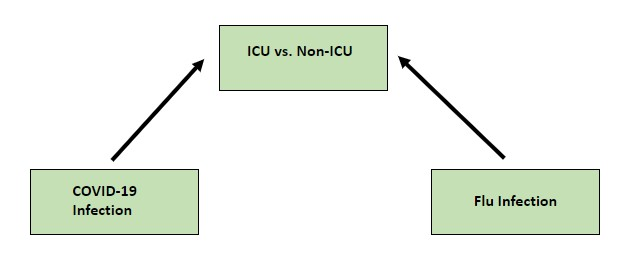
\includegraphics[scale = 0.6]{figures/covidflucollider}
	\end{figure}
\end{frame}

\begin{frame}{
\includegraphics[scale = 0.015]{figures/technical}M-Bias}
	We also said a collider can be \textcolor{blue}{associated with} the exposure and \textcolor{blue}{associated with} the outcome 
	\medskip
	
	In fact, we excluded this kind of variable from our definition of confounder
	
	\medskip
	Why?
\end{frame}

\begin{frame}{
\includegraphics[scale = 0.015]{figures/technical}M-Bias}
	Here mother's diabetes is a collider
	\begin{figure}
	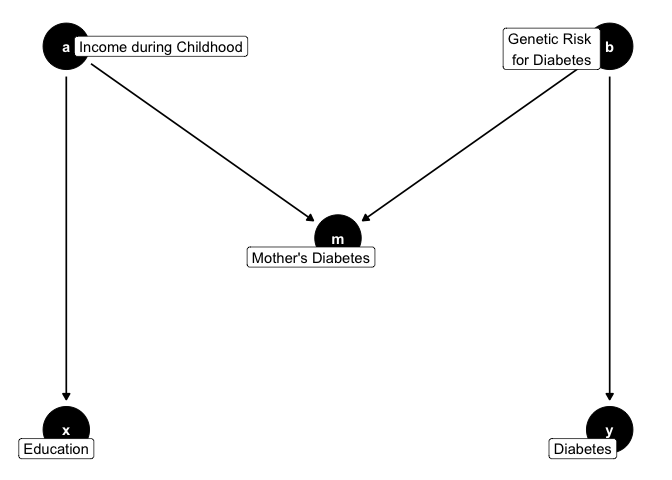
\includegraphics[scale = 0.4]{figures/m_bias}	
		\end{figure}
\footnote{\url{https://cran.r-project.org/web/packages/ggdag/vignettes/bias-structures.html}}
\end{frame}

\end{document}